\color{white}
\pagecolor{black_background}

\tableofcontents
\newpage

\chapter{SISTEMAS DE LOSAS POSTENSADAS}
\newpage

\section{USO DE LOSAS POSTENSADAS EN EDIFICACIONES}

Esta es una imagen que se hizo en Bolivia, en el departamento de
Potosi. donde se tenia la idea de eliminar las dos columnas marcadas
de color rojo.

\begin{figure}[H]
\centering
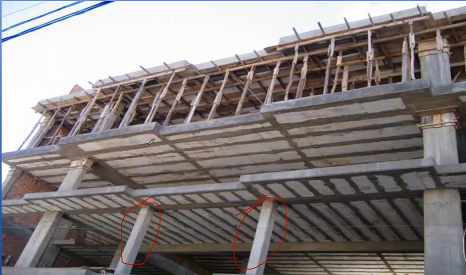
\includegraphics{1.png}
\end{figure}

En la siguiente imagen se muestra un esquema de la primera losa 
de hormigon armado y luego una losa postensada, para precindir 
de las columnas en las losas superiores. Es decir por razones
de funcionalidad se queria hacer salon de fiestas, Es decir que
se tiene que verificar que cumpla con la vibración permitida.

\begin{figure}[H]
\centering
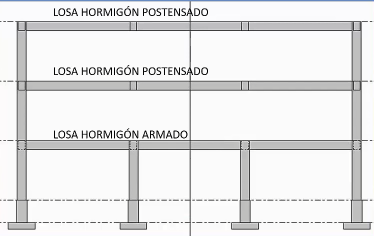
\includegraphics{2.png}
\end{figure}

A travez de los cables y los anclajes se logra generar una carga
opuesta al peso propio. como se muestra en la siguiente imagen

\begin{figure}[H]
\centering
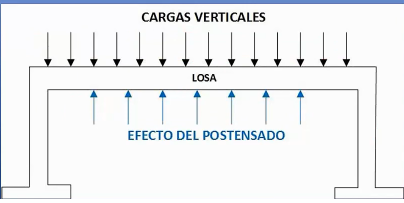
\includegraphics{3.png}
\end{figure}

\section{MATERIALES}

\begin{itemize}
	\item HORMIGON, ACERO (barras corrugadas)
	\item CABLE PARA POSTENSADO
	\item ANCLAJES
\end{itemize}

En la siguiente imagen se muestra el cable para puentes, que coloquialmente
le decimos cable pelado. La tecnologia que se usa en la mayoria de los puentes,
en las vigas que se postensan se llama "sistema adherido",
en este curso vamos a ver el "sistema no adherido".

\begin{figure}[H]
\centering
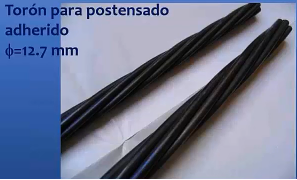
\includegraphics{4.png}
\end{figure}

Para el "sistema no adherido" se utiliza el mismo cable pero esta recubierto
con grasa y una capa de plastico.

\begin{figure}[H]
\centering
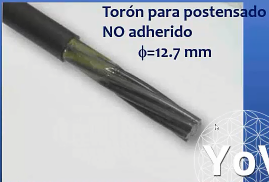
\includegraphics{5.png}
\end{figure}

El diametro que más se utiliza es el de media pulgada o de 12.7 mm, en los catalogos
de los fabricantes se puede encontrar direfentes diametros pero el de diametro 12.7mm
es el mas comercial.

\section{DETALLE CABLE PARA POSTENSADO NO ADHERIDO}

\begin{figure}[H]
\centering
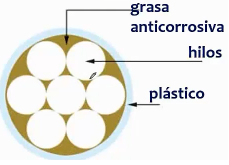
\includegraphics{6.png}
\end{figure}

Se puede apreciar que es un toron de siete hilos recubierto con una capa de plastico
y engrasado, nosotros le decimos engrasado y envainado.

\begin{figure}[H]
\centering
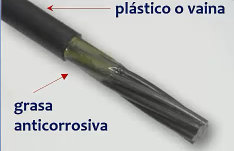
\includegraphics{7.png}
\end{figure}

Una vez que se realiza el tesado en una losa postensada no se requiere inyección
de lechada

\section{DETALLE CABLE PARA POSTENSADO NO ADHERIDO}

video en espera min 14:16

